\documentclass[letterpaper,10pt]{article}
\usepackage{times}
\usepackage{helvet}
\usepackage{courier}
\usepackage{txfonts}
\usepackage{array}
\newcolumntype{P}[1]{>{\centering\arraybackslash}p{#1}}
\usepackage{float}
\frenchspacing
%\setlength{\pdfpagewidth}{8.5in}
%\setlength{\pdfpageheight}{11in}
\usepackage{indentfirst}
%used for pseudocode
\usepackage{algpseudocode}

%used to make charts
\usepackage{pgfplotstable}
\usepackage{pgfplots}

%used for mathematical notation
\usepackage{amsfonts}

%used to control spacing in table captions
\usepackage{subfig}

%used to import images
\usepackage{graphicx}

%used to specify table placement
\usepackage{float}

% Make it so lists don't have extra line spacing:
\usepackage{enumitem}
\setlist{noitemsep}

\usepackage{hyperref} % for \url

% For nice, customizable code listings:
\usepackage{listings}
\lstset{ %http://stackoverflow.com/questions/586572/make-code-in-latex-look-nice
	language=Python,
	basicstyle=\footnotesize,       % font size
	numbers=left,                      % where line numbers appear
	numberstyle=\footnotesize,   % size of line numbers
	stepnumber=1,                    % how often line numbers appear
	numbersep=5pt,                   % space between line numbers and code
	showstringspaces=false,       % whether or not to show a _ in strings
	frame=single,                       % what kind of frame should be around the code
	xleftmargin=1.5em,
	xrightmargin=1em,
	framexleftmargin=0em,
	%rulecolor=\color{black},         % for the frame
	tabsize=2,                             % set the number of spaces for tabs
	breaklines=true,                     % set whether or not linebreaking should occur
	breakatwhitespace=true,          % set whether or not linebreaking should occur only at spaces
	lineskip={-1.0pt}
	%commentstyle=\color{mygreen}, % color for code comments
	%numberstyle=\color{mygray}, % style for line numbers
}

\renewcommand{\today}{}
\renewcommand{\baselinestretch}{2.0}
%\usepackage{plain} % for the bibliography

\usepackage{ragged2e}
\usepackage[utf8]{inputenc}

\title{House Prices Prediction}
\author{Anh Le, Eric Spehlmann }
\date{December 2019}

\begin{document}
\maketitle
\renewcommand{\thesection}{\Roman{section}} 
\section{Abstract}
The housing market is a complex domain that is influenced by multiple variables impacting the price of individual houses. Machine learning has been applied to the local and national housing market to create models that are used to guide appraisers, sellers, and buyers of houses. The data set used in this model represents a suburban community in Ames Iowa. The goal of the project was to experiment with data analysis methods to establish the best estimator of housing prices.  The analysis used in this project ranged from varying preprocessing, algorithms, parameterization, and attribute strategies. After, intensifying attention to attribute selection based on size, age, quality, and location, the model became increasingly more accurate. The research finished with a working model that produced an accuracy of 91\% using gradient boosting regression as the estimator.	

\section{Introduction}
The data used for this particular Kaggle competition contained data on houses in Ames Iowa and the selling price of the house. Each data point had 81 attributes describing almost all information of the house. The housing data included 43 categorical attributes 38 numerical attributes. This would later represent a problem when dealing with the immense volume of categorical data. The training set contained 1460 elements while the testing set contained 1459. Knowing the particulars of the data was helpful; however, further understanding of the housing domain led to better understanding of the dataset. Housing prices are greatly determined by the location of the house, the size of the house, time sold, and condition of the house. These insights were crucial in preprocessing and selecting predictors for the algorithm. The values that correlated most directly with sales price were selected using pandas .corr method to obtain the top 10 attributes. These attributes described what was predicted to affect the house price. After forming an educated understanding of the data set, data cleaning was the next step in getting the data ready for fitting an algorithm.  

\begin{table}[H]
\centering
\begin{tabular}{ |p{4cm}|P{4cm}| } 
 \hline
  & Correlation \\ 
 \hline
 SalePrice & 1.000000 \\ 
 \hline
 OverallQual & 0.790982 \\ 
 \hline
 GrLivArea & 0.708624 \\ 
 \hline
 GarageCars & 0.640409 \\ 
 \hline
 GarageArea & 0.623431 \\ 
 \hline
 TotalBsmtSF & 0.613581 \\ 
 \hline
 1stFlrSF & 0.605852 \\ 
 \hline
 FullBath & 0.560664 \\ 
 \hline
 TotRmsAbvGrd & 0.533723 \\ 
 \hline
 YearBuilt & 0.522897 \\ 
 \hline
\end{tabular}
\caption{Top 10 Attributes Relating to Sale Prices}
\label{table:1}
\end{table}

\section{Pre-Processing}
The data proved to have missing values in both the testing and training set. First, we eliminated attributes with 90\% of their data missing using the thresh parameter in the \href{https://towardsdatascience.com/how-to-handle-missing-data-8646b18db0d4}{\it dropna()} method with {\it thresh} parameter, provided by pandas. This made matters less tricky when deciding to fill those missing values. Next, the attributes were divided into numerical and categorical data. To fill in the values of the missing numerical data, the mean was calculated from the training set and was imputed into the row. This ensured no chance of data leakage to the testing set.\par
Categorical data was handled using advice from the website “towards data science”; which detailed filling the missing categorical data with the mode (highest frequency). If the categorical data had more than 10 missing values, the values were set to ‘None’. Once missing values were filled or removed, attribute engineering was attempted to improve the model in the future. \par
Attribute engineering is the process by which new attributes are used to encapsulate multiple attributes or describe a feature that could be interpreted from values. The attributes engineered for the model included, total bath number, total square footage, and age. Total baths was created by adding the number of baths, counting a full bath as one and a half bath as 0.5, respectively. This allowed for the one attribute to encapsulate 4. The total square footage was created to sum the total area of the house. Age was devised by subtracting the year built from 2019 to get years old. Lastly, the year remodeled attribute was manipulated to be “remodeled” which contained a 1 or 0 if the house was remodeled.\par
Encoding of categorical information varied based on the attribute, location and condition were handled similarly. After investigating the most expensive neighborhoods, by summing sales prices from neighborhoods using the {\it groupby()} method provided by pandas, a map was created to change the categories into ordinal values. This same concept was used for condition which represented key location information. Other categorical attributes represented ordinal values that could be handled with similar cases. Many of the qualitative attributes used varying scales of “excellent, good, avg, poor”. This presented an opportunity to  map the strings to a scale of 1-4 or 1-6 depending on the particular scale. \par
Lastly, \href{https://towardsdatascience.com/smarter-ways-to-encode-categorical-data-for-machine-learning-part-1-of-3-6dca2f71b159} {binary encryption and one hot encoding} were incorporated into the data set to encrypt categorical data. The roof style seemed of minor importance, but figuring certain roofs were better for the cold weather in Ames, it was decided to incorporate it. Binarization using Sklearn Binarizer was used to create labels for the roofs. This only affected the model’s variance if using gradient boosting. In addition to binary encoding, one hot encoding was used to encode the foundation attribute. Foundation represents an expensive construction aspect of the house. Using the pandas {\it get\_dummies()} method, foundation was encrypted. 

    \textbf{Algorithms:} \par
\href{https://www.analyticsvidhya.com/blog/2017/06/a-comprehensive-guide-for-linear-ridge-and-lasso-regression/} {Linear regression, linear ridge, lasso}, and \href{https://scikit-learn.org/stable/modules/generated/sklearn.ensemble.GradientBoostingClassifier.html}{gradient boosting} were all experimented with to determine which created the best model for predicting housing price. All the models were linear regression models except gradient boosting were linear regressors. Linear regression was used as a guiding light throughout the project. The preprocessing models used focused largely on creating all numeric values so that the linear models could be fitted. 
Linear ridge is a type of linear regressor that works on data sets with sparse information. Thinking the data set was considerably small, ridge was used to get started with hyper tuning. Ridge regression implements a penalty term that enforces a simpler model to be developed. The results were marginally better than linear regression.\par

$$\sum_{i=1}^{M} (y_i - y_i)^2 = \sum_{i=1}^{M}(y_i - \sum_{j=0}^{p} (w_j * x_{ij})^2 + \lambda \sum_{j=0}^{p} w^2_j $$
\begin{center} Cost function for Ridge Regression
\end{center}

$$\sum_{i=1}^{M} (y_i - y_i)^2 = \sum_{i=1}^{M}(y_i - \sum_{j=0}^{p} (w_j * x_{ij})^2 + \lambda \sum_{j=0}^{p} |w_j| $$
\begin{center} Cost function for Lasso Regression
\end{center}

Both ridge and lasso implement regularization, a method used to limit individual coefficients from weighing more than others, preventing overfitting. Lasso shrinks the number the attributes to a mean to avoid complexity. Lasso eventually would return a cv score of 83\%. \par
Lastly, gradient boosting was used to venture away from linear regression. Gradient boosting regressor represents an ensemble, an algorithm that produces multiple groups of models to converge to one best fitting model. However, with this power comes the increased potential of over fitting. The learning rate was key in producing a model that did not overfit the data.\par
    \textbf{Hyperparameterization:} \par
Trying to create a universal tuning method for hyperparameterizing the algorithms took trial and error. Eventually, using ranges of values and mapping each value to a new algorithm produced an easy way to test tuning values. Linear ridge and lasso were manipulated using the alpha value. 1000 alpha values range from 0.01 to 1 with a step of 0.01, were used to graph varying ‘accuracies’. The gradient boost regressor was tuned with the same process however the learning rate was adjusted instead. Eventually,  optimal values were obtained.  

\begin{figure}[H]
    \centering
    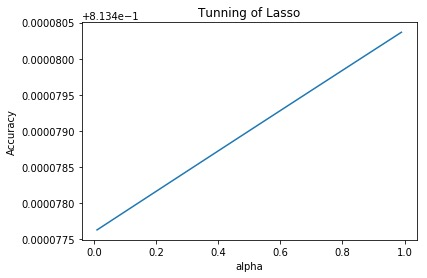
\includegraphics[scale=0.7]{Lasso.jpeg}
    \caption{Relative Accuracies Corresponding to Alpha}
    \label{fig:Content-basedRecommender}
\end{figure}
\begin{figure}[H]
    \centering
    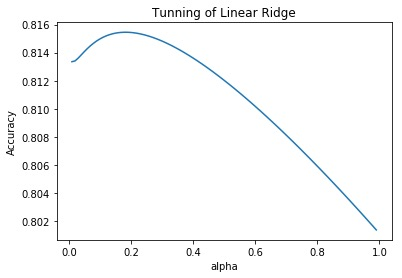
\includegraphics[scale=0.7]{Ridge.jpeg}
    \caption{Relative Accuracies Corresponding to Alpha}
    \label{fig:Content-basedRecommender}
\end{figure}
\begin{figure}[H]
    \centering
    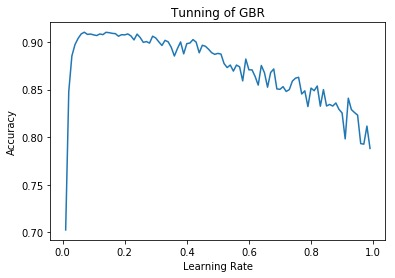
\includegraphics[scale=0.7]{TunningGBR.jpeg}
    \caption{Relative Accuracies Corresponding to Learning Rate}
    \label{fig:Content-basedRecommender}
\end{figure}

    \textbf{Results:} \par
After hyper tuning the models, predictions started to become more accurate.  Linear ridge, and lasso had similar r2 scores but varied widely in their kaggle score. Lasso out performed ridge in the kaggle test, this could be due to the difference in score calculations between the average variance and mean squared error.  Gradient Boost had the best results of the three models used in the kaggle competitions. The  r2 score was 0.91 kaggle score resulted in 0.153. 

\begin{table}[H]
\centering
\begin{tabular}{ |p{3cm}|p{3cm}|p{2cm}|p{2cm}| } 
 \hline
  Model & Tuning Parameter & Accuracy (r2) & Kaggle Score \\ 
 \hline
 Linear Ridge & Alpha: 0.069 & 0.815 & 0.783 \\ 
 \hline
 Lasso & Alpha: 0.99 & 0.813 & 0.177 \\ 
 \hline
 Gradient Boosting & Learning Rate: 0.069 & 0.911 & 0.153 \\ 
 \hline
\end{tabular}
\caption{Comparation of CV scores between different models}
\end{table}

     \textbf{Analysis:} \par
Concluding from the results, gradient boosting had comparative edge on the other models. Boosting is a powerful technique that uses multiple models to improve upon the errors made by previous models. This is clearly an advantage over linear regression; Although, requiring more processing power to run. Secondly, hyper tuning was crucial in creating accurate scores. The graphs above illustrate the high drop offs in accuracy due to over or under stepping the hyper parameter. 

\section{Conclusion}
The preprocessing seemed most important in creating accurate models. Key factors affecting the models seems to be missing values, and predictors used. Given the following predictors related to location, size, age, and quality of the house, the algorithms had enough information to create semi accurate results. Values that correlated highly with price played an important role in effective preprocessing. Linear regression worked well with numeric data; although, ultimately they didn't have enough information alone without using categorical inputs. Using an ensemble, gradient boosting regressor, the model was able to produce the most accuracy. Concludingly, knowing the domain of the data is most important at intuiting a beautiful model. 

\begin{thebibliography}{999}

\bibitem{lamport94}
Swalin, Alvira,
"How to Hanndle Missing Data",
\emph{Medium}.
Towards Data Science, 19 Mar. 2018,
https://towardsdatascience.com/how-to-handle-missing-data-8646b18db0d4
  
\bibitem{lamport94}
Hale, Jeff,
"Smarter Ways to Encode Categorial Data for Machine Learning",
\emph{Medium}.
Towards Data Science, 16 July. 2019,
https://towardsdatascience.com/smarter-ways-to-encode-categorical-data-for-machine-learning-part-1-of-3-6dca2f71b159

\bibitem{lamport94}
Jain, Shubham,
"Linear, Ridge and Lasso Regression Comprehensive Guide for Beginners.",
\emph{Analytics Vidhya}.
17 Sept. 2019, www.analyticsvidhya.com/blog/2017/06/a-comprehensive-guide-for-linear-ridge-and-lasso-regression/.

\bibitem{lamport94}
"“3.2.4.3.5. Sklearn.ensemble.GradientBoostingClassifier¶.”,
\emph{Scikit}, 
scikit-learn.org/stable/modules/generated/sklearn.ensemble.GradientBoostingClassifier.html.

\end{thebibliography}

\end{document}
